\begin{figure}
  \centering
  \vspace{-0.25cm}
  \begin{tikzpicture}
    \node at (0, 1.1){
      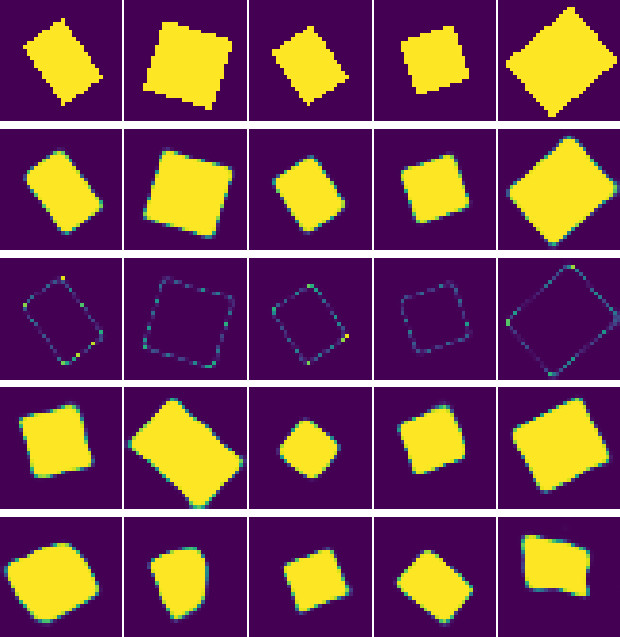
\includegraphics[width=6cm]{experiments/3d/vae_occ/easy_15/results_0}
    };
    \node at (0, -1.1){
      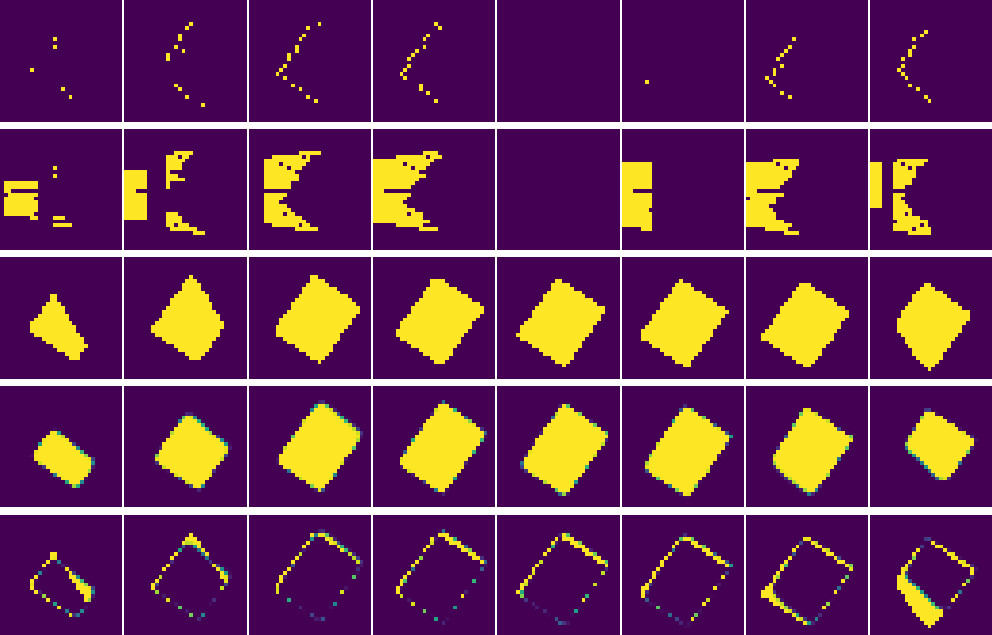
\includegraphics[width=6cm]{experiments/3d/vae_occ/easy_15/results_1}
    };
    
    \draw[-,dashed] (3.25, -8) -- (3.25,3);
    
    \node at (6.5, 0){
      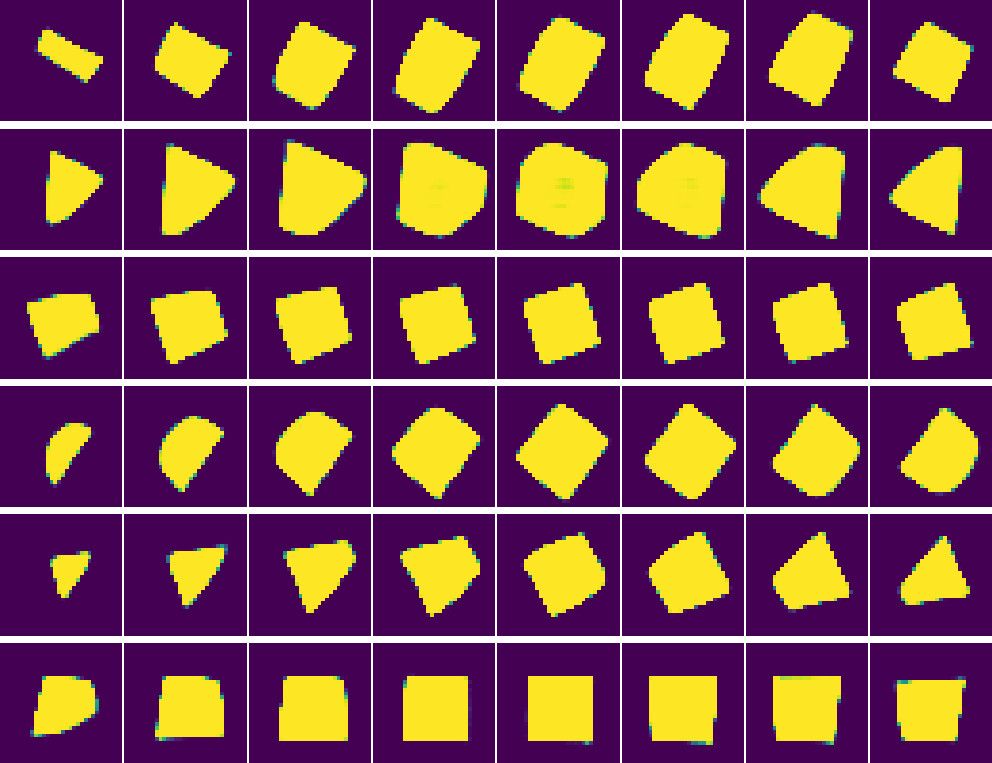
\includegraphics[width=6cm]{experiments/3d/vae_occ/easy_15/random}
    };
    
    \node at (10,0) {
      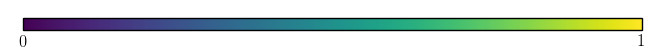
\includegraphics[height=5cm]{experiments/3d/vae_occ/easy_15/colorbar}
    };
    
    \node at (0, 3) {\begin{tabular}{c}reconstruction\\occupancy\end{tabular}};
    \node at (6.5, 3) {\begin{tabular}{c}random samples\\occupancy\end{tabular}};
    
    \draw[-,dashed] (-3.5, -2.5) -- (10, -2.5);
    
    %\node at (-3.5,-5) {
    %  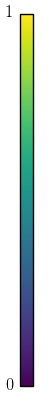
\includegraphics[height=5cm]{experiments/3d/vae_occ_sdf/colorbar_0}
    %};
    
    \node at (0, -5){
      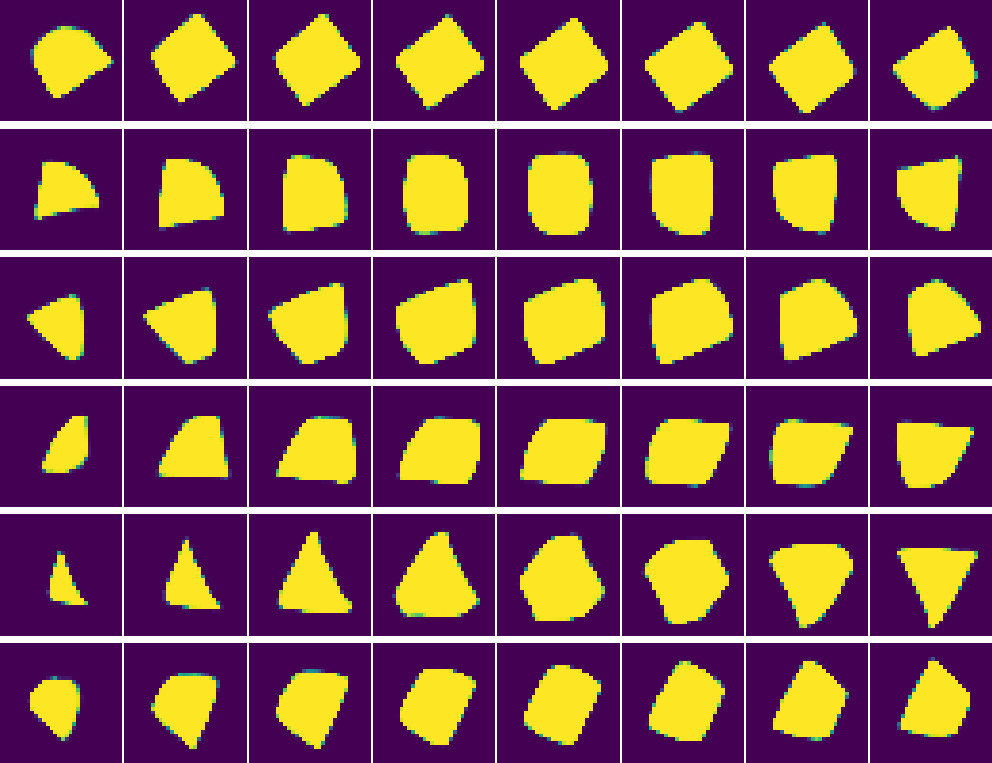
\includegraphics[width=6cm]{experiments/3d/vae_occ_sdf/easy_15/random_0_0}
    };
    
    %\draw[-,dashed] (3.25, -3) -- (3.25,3);
    
    \node at (6.5, -5){
      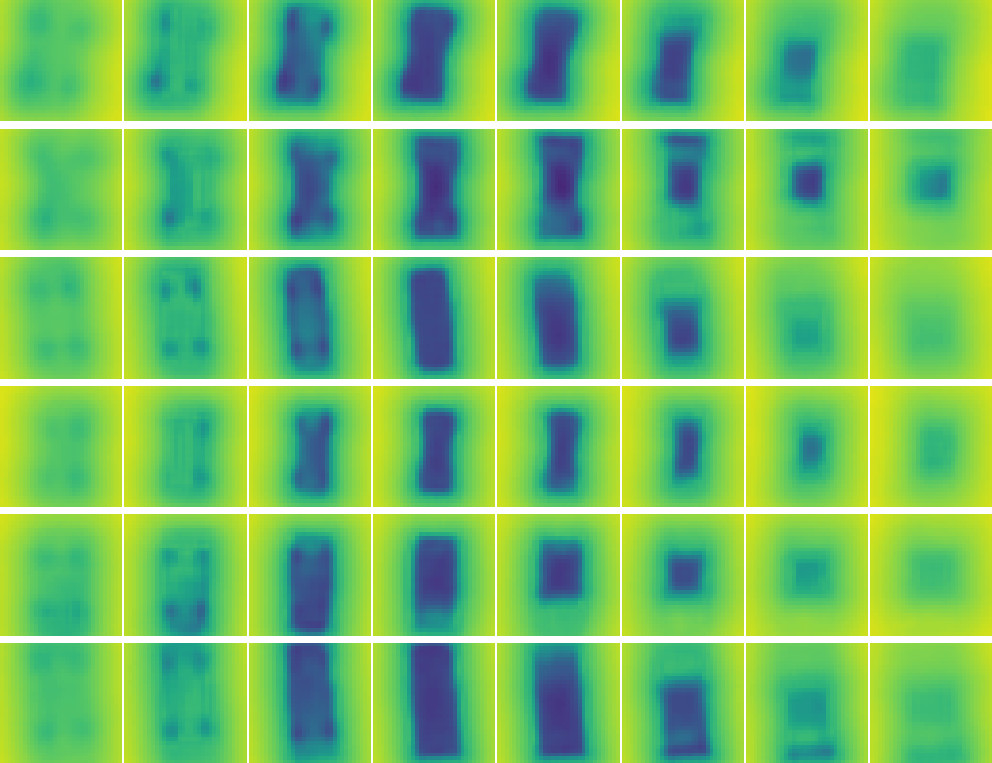
\includegraphics[width=6cm]{experiments/3d/vae_occ_sdf/easy_15/random_0_1}
    };
    
    \node at (10,-5) {
      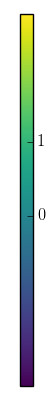
\includegraphics[height=5cm]{experiments/3d/vae_occ_sdf/colorbar_1}
    };
   
    \node[rotate=90] at (-3.75, 0) {\begin{tabular}{c}predicting occupancy only\end{tabular}};
    \node[rotate=90] at (-3.75, -5) {\begin{tabular}{c}predicting occupancy and\\signed distance functions\end{tabular}};
   
    \node at (0, -8) {\begin{tabular}{c}random samples\\occupancy\end{tabular}};
    \node at (6.5, -8) {\begin{tabular}{c}random samples\\signed distance functions\end{tabular}};
  \end{tikzpicture}
  
  % TODO short caption
  \caption{Qualitative results for the trained \VAE shape prior with $Q = 15$ on the 3D cuboids dataset.
  We consider two models; one trained on occupancy only and one trained on both occupancy and
  signed distance functions. In the first case, we show reconstruction results on the left and
  random samples on the right. For the latter case, we show only random samples for both modalities.
  In all cases we show horizontal slices, \ie heights $8 + 2i$ for $0 \leq i < 8$. For random samples
  in the occupancy only case, we complement the results with 3D visualizations in Figure
  \ref{fig:experiments-3d-vae-qual-2}.}
  \label{fig:experiments-3d-vae-qual-1}
\end{figure}
\begin{figure}
  \centering
  \vspace{-0.25cm}
  \hspace*{-1cm}
  \begin{tikzpicture}
    \node at (0, 0) {
      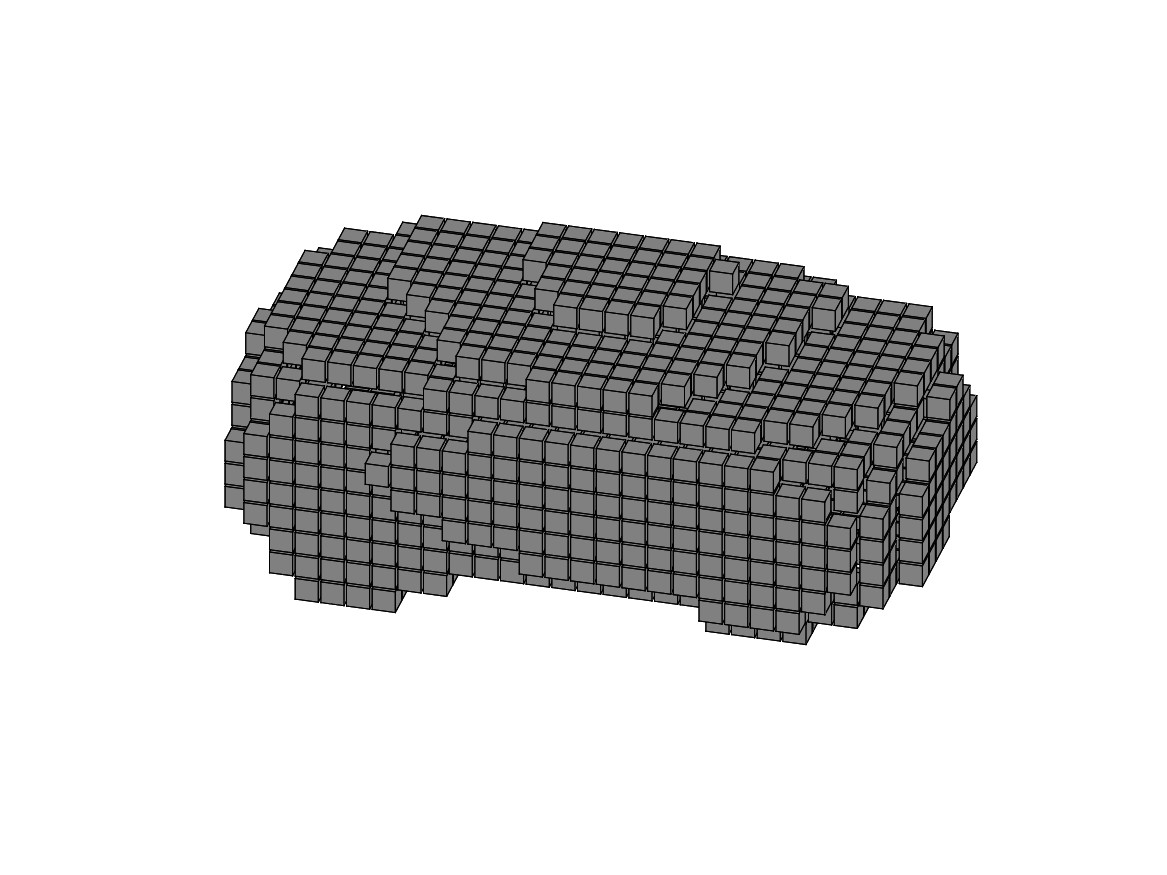
\includegraphics[width=2.5cm,trim={2cm 1cm 2cm 1cm},clip]{experiments/3d/vae_occ/easy_15/0_random_15}
    };
    \node at (2.5, 0) {
      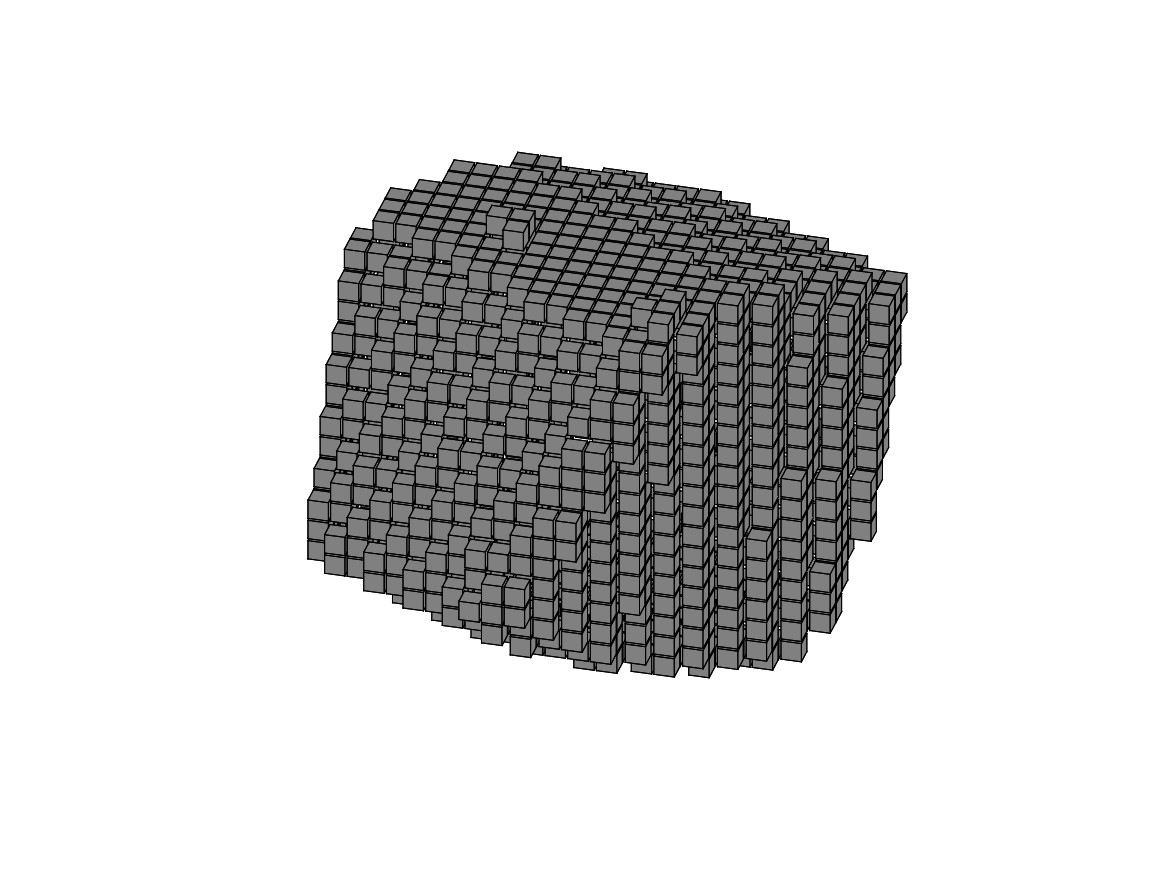
\includegraphics[width=2.5cm,trim={2cm 1cm 2cm 1cm},clip]{experiments/3d/vae_occ/easy_15/0_random_105}
    };
    
    \draw[-,dashed] (4,-1.5) -- (4, 1.5);
    
    \node at (5.5, 0) {
      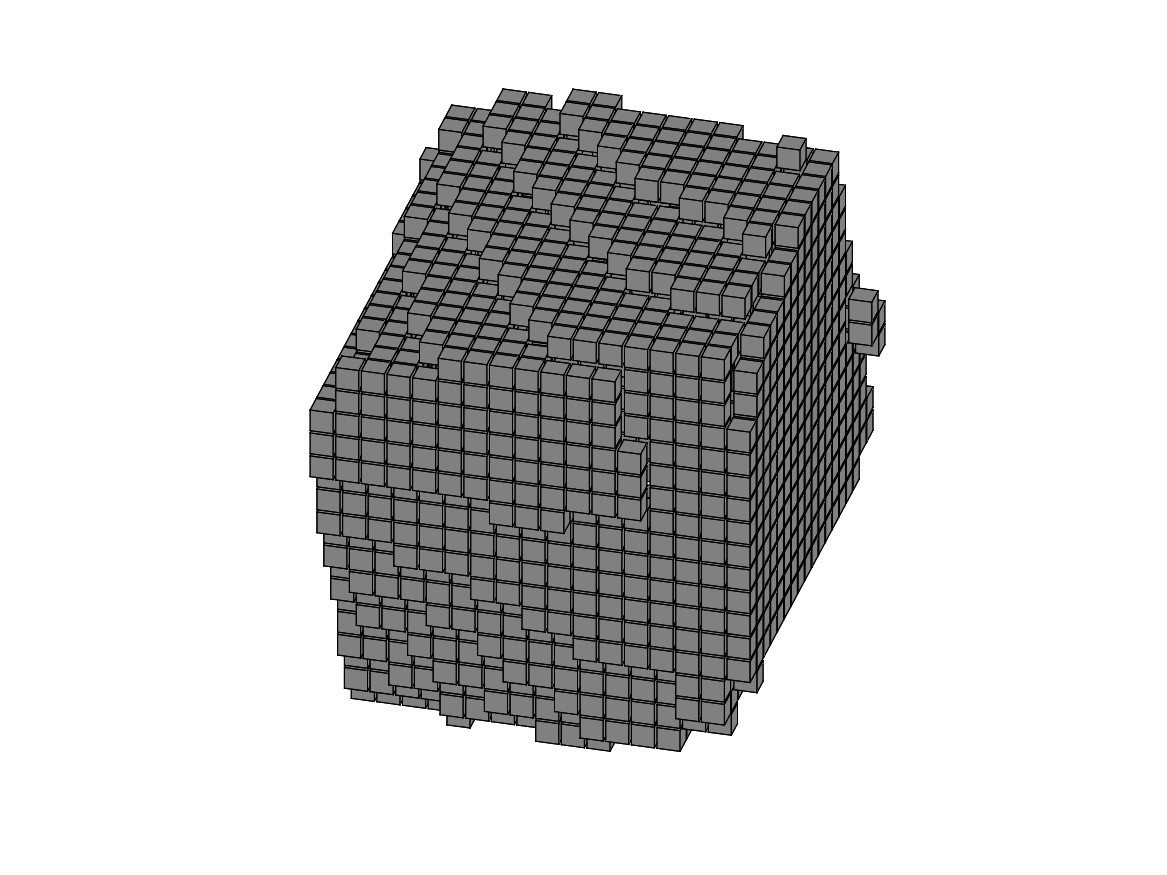
\includegraphics[width=2.5cm,trim={2cm 1cm 2cm 1cm},clip]{experiments/3d/vae_occ/easy_15/5_random_15}
    };
    \node at (8, 0) {
      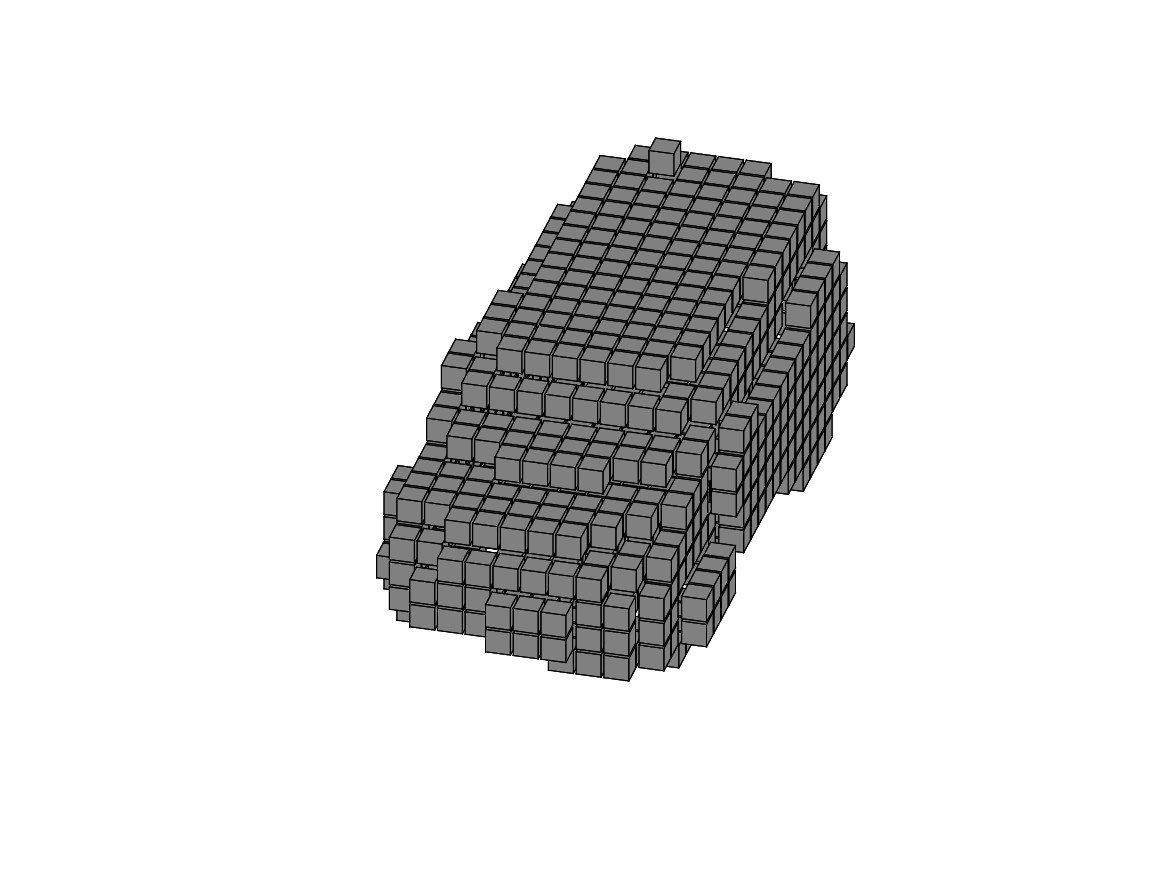
\includegraphics[width=2.5cm,trim={2cm 1cm 2cm 1cm},clip]{experiments/3d/vae_occ/easy_15/5_random_105}
    };
    
    \draw[-,dashed] (9.5,-1.5) -- (9.5, 1.5);
    
    \node at (11, 0) {
      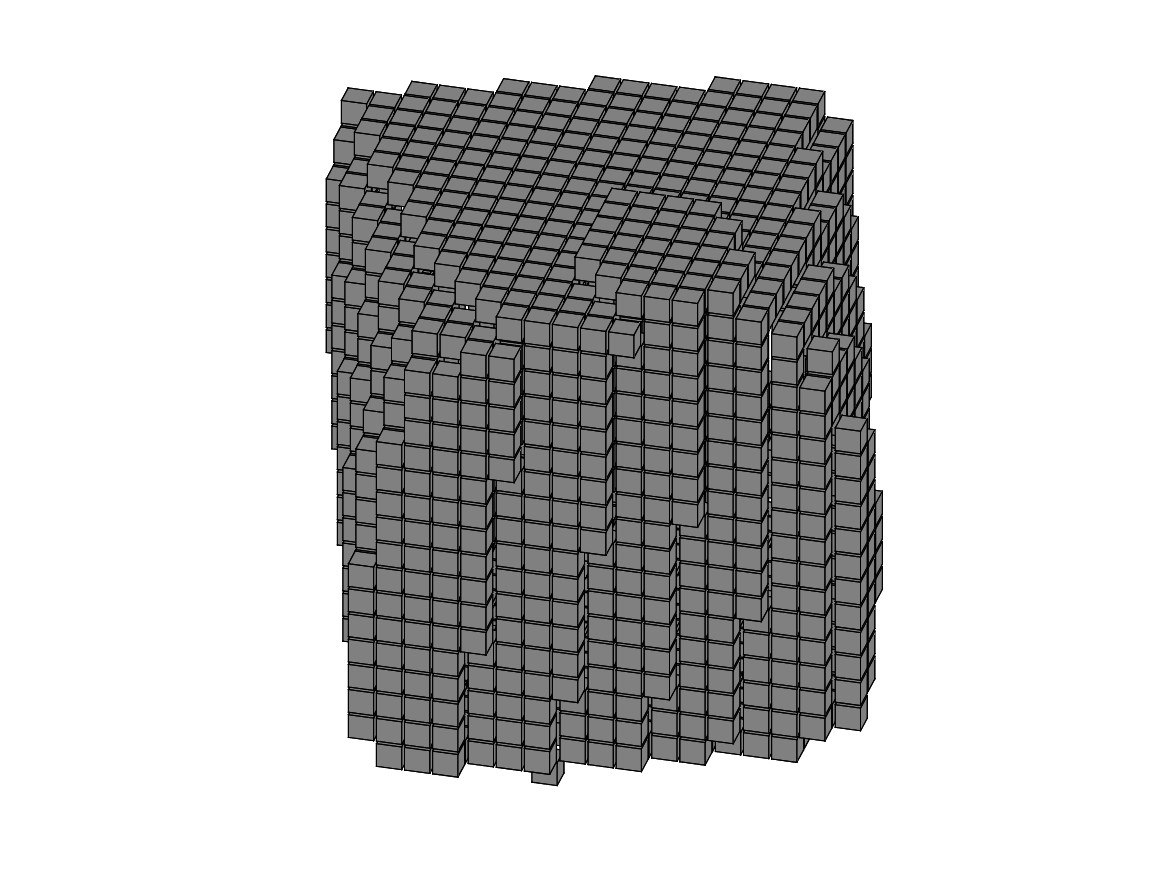
\includegraphics[width=2.5cm,trim={2cm 1cm 2cm 1cm},clip]{experiments/3d/vae_occ/easy_15/2_random_15}
    };
    \node at (13.5, 0) {
      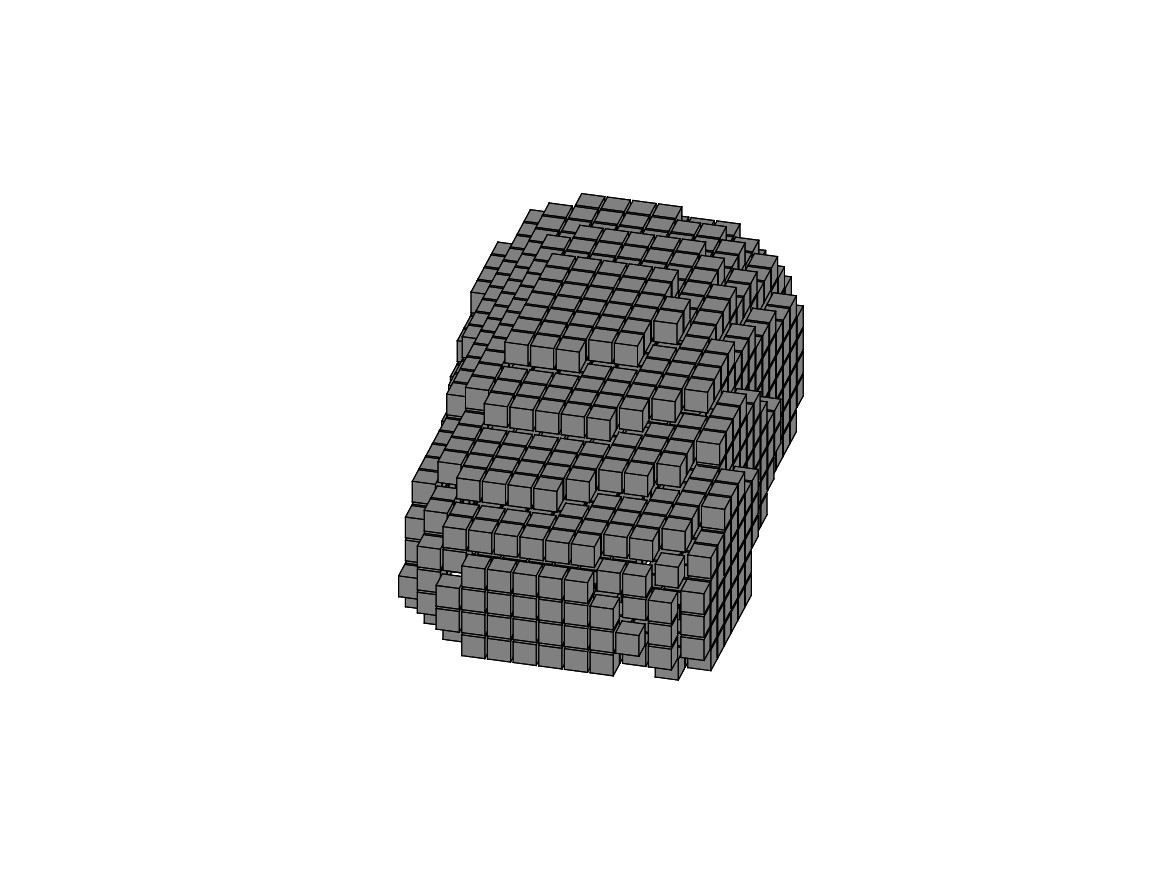
\includegraphics[width=2.5cm,trim={2cm 1cm 2cm 1cm},clip]{experiments/3d/vae_occ/easy_15/2_random_105}
    };
  \end{tikzpicture}
  \caption{Three random example of the \VAE shape prior with $Q = 15$ on the 3D cuboids dataset
  trained on occupancy only. In all three cases, we show two different viewpoints. We find that all
  three examples resemble cuboids. We also note that the \VAE has no difficulties predicting sharp corners
  and edges.}
  \label{fig:experiments-3d-vae-qual-2}
\end{figure}
